% Chapter Template

\chapter{Deep Learning} % Main chapter title

\label{Chapter4} % Change X to a consecutive number; for referencing this chapter elsewhere, use \ref{ChapterX}

We lay the foundation for deep learning, because we want to explore the application of deep learning in arbitrage teory specially to option pricing in the next chapter. Deep learning experiences a renaissance, because of the technology improvements in hardware and software. The collection of data has also significant improved the field. Deep learning is a specialized field in machine learning, where you focus on a special architecture of models. Like in machine learning the basic components of a deep learning algorithm are a dataset, cost function, optimazation algorithm and a model. E.g. in the lsm method we assumed the model was gaussian, dataset was the simulated paths, the loss function was the mean square error and the optimazation algorithm was solving the normal equations. Deep learning is about studying neural networks which allows for greater flexiblity than standard methods like linear regression. "Deep" comes from that a neural network consists of multiple layers, where the depth tells you how many layers the network has.\\

All the algorithms applied will be within supervised learning, where we try to fit the best between the features and the response variable. Furthermore all our algorithms will be based on the multilayer perceptrons (MLPs) for regression, hence it will also be the main focus.

%----------------------------------------------------------------------------------------
%	SECTION 1
%----------------------------------------------------------------------------------------

\section{Multilayer Perceptrons}
The goal of the multilayer perceptrons (MLPs) is to approximate a function $f^*(x)$, where the MLPs defines a mapping $f(x;\theta)$ to approximate $f^*(x)$. The task is to find the best $\theta$ such that the approximatation $f(x;\theta)$ is close to the targets provided for some defined objective function. To build the network we start with zooming in on a single neuron, which is one node of a directed acyclic graph (see figure \ref{fig:multilayer-perceptron}). Note the MLPs is called a feedforward network, because all the connections between the neurons are directed such that the network forms a directed acyclic graph.

%-----------------------------------
%	SUBSECTION 1
%-----------------------------------
\subsection{A Single Neuron}\label{singleNeuron}
The single neuron has a number P features of inputs $x_p$ and one output $\hat{y}$ (see figure \ref{fig:singleNeuron}). 

\tikzset{%
  every neuron/.style={circle,draw,minimum size=1cm},
  neuron missing/.style={draw=none,scale=4,text height=0.333cm,execute at begin node=\color{black}$\vdots$},
}
\begin{center}
    \begin{figure}[h]
        \begin{tikzpicture}[
        		init/.style={
 				draw,
  				circle,
  				inner sep=2pt,
  				font=\Huge,
  				join = by -latex
			},
			squa/.style={
  				draw,
  				inner sep=2pt,
  				font=\Large,
  				join = by -latex
			},
			start chain=2,node distance=13mm
			]
			\node[on chain=2] 
			  (x2) {$x_2$};
			\node[on chain=2,join=by o-latex] 
			  {$w_2$};
			\node[on chain=2,init] (sigma) 
			  {$\displaystyle\Sigma$};
			\node[on chain=2,squa,label=above:{\parbox{2cm}{\centering Activate \\ function}}]   
			  {$g$};
			\node[on chain=2,label=above:Output,join=by -latex] 
			  {$y$};
			\begin{scope}[start chain=1]
			\node[on chain=1] at (0,1.5cm) 
 				(x1) {$x_1$};
			\node[on chain=1,join=by o-latex] 
				  (w1) {$w_1$};
			\end{scope}
			\begin{scope}[start chain=3]
				\node[on chain=3] at (0,-1.5cm) 
				  (x3) {$x_3$};
				\node[on chain=3,label=below:Weights,join=by o-latex] 
			 	 (w3) {$w_3$};
			\end{scope}
			\node[label=above:\parbox{2cm}{\centering Bias \\ $w_0$}] at (sigma|-w1) (b) {};

			\draw[-latex] (w1) -- (sigma);
			\draw[-latex] (w3) -- (sigma);
			\draw[o-latex] (b) -- (sigma);

			\draw[decorate,decoration={brace,mirror}] (x1.north west) -- node[left=10pt] {Inputs} 				(x3.south west);
        \end{tikzpicture}
        \caption{A single neuron}
        \label{fig:singleNeuron}
    \end{figure}
\end{center}

The function from inputs to output for a single neuron is:
\begin{align}   
\hat{y}=g(w_0 + \bm{x}^T \bm{w}) \quad where \quad \bm{w}=\begin{pmatrix}
x_1 \\
\vdots\\
x_p
\end{pmatrix} \quad and \quad \bm{w}=\begin{pmatrix}
w_1 \\
\vdots \\
w_p
\end{pmatrix}
\end{align}
The $\matr{W}$ is the weight matrix and $w_0$ is the bias term. The term inside the function g is the activation of the neuron and it is denoted:
$$a= w_0 + \bm{x}^T \bm{w}$$
The function g is the activation function and it is essential for the flexibility of the MLPs. There exits numerous of activations function only the imagination is the limit. We will list the most common and discuss the them \parencite{Mackay18}.


%-----------------------------------
%	SUBSUBSECTION 1
%-----------------------------------
\subsubsection{Activation functions}
Activation functions are important feature for neural network, because they allow for non-linearities and flexibility. Activation functions apply a non-linear transformation and decide whether a neuron should be activated or not. Without activation functions or the identity function $g(a)=a$ the whole network would essentially be a linear regression model. Some popular activation functions:
\begin{enumerate}
\item[•] Sigmoid function: $g(a)=\frac{1}{1+\exp(-a)}$\\
This is the traditional choice, also called logistic function. Popular in classification but can suffer from vanishing gradient (TODO) in deep learning.
\item[•] Hyperbolic tangent function: $g(a)=\frac{e^a-e^{-a}}{e^a+e^{-a}}$\\
A scaled and shifted sigmoid function and likewise suffers from the vanishing gradient problem. The range is $(-1,1)$ and centered at zero. Often used for hidden layers.
\item[•] ReLU function: $g(a)=\max(0,a)$.\\
Rectified Linear Unit is one of the most popular choices since is does not suffer from the vanishing gradient problem. The MLPs often becomes more sparse because it sets some features to zero. It is claimed that ReLU learns muliple times faster than both the hyberbolic tangent and the sigmoid function.
\item[•] Leaky ReLU function better version than Relu:  \[ g(a)=
    \begin{dcases}
        a & if \ a \geq 0 \\
        \alpha \cdot x & otherwise \\
    \end{dcases}
\]\\
The fact that ReLU can have some hidden covariates that is zero can be an advantage, but also a disadvantage since some neurons may die out as all the neurons are zero. The Leaky ReLU is designed to give such neurons a chance to get back into action, but not too easily, so $\alpha>0$ is chosen small ( typical $\alpha=0.01$ ) 

\item[•] ELU - exponential linear unit:  \[ g(a)=
    \begin{dcases}
        a & if \ a \geq 0 \\
        \alpha(\exp(a)-1) \cdot x & otherwise \\
    \end{dcases}
\]\\
Like the Leaky ReLU the ELU is designed to avoid the dead ReLU problem. 
\end{enumerate}

With a understanding of a single neuron we continue to the architecture of a MLPs \parencite{Goodfellow-et-al-2016} \parencite{Mackay18}.


%-----------------------------------
%	SUBSECTION 2
%-----------------------------------
\subsection{Architecture Of MLPs}
A MLPs constist of a input layer, where all $p$ features enters, $L$ hidden layers, and an output layer. Each hidden layer and the output layer consists of multiple neurons, where the width of the layer is the number of neurons in that layer ($m^l$) (see figure \ref{fig:multilayer-perceptron}). The networks inputs are called the input layer, the output layer is the output of the neural network. The layers between the input and output layer are hidden layers. This could be an explanation why the field is called Deep learning, because we a deep structure of layers. In each hidden layer a linear combination of the featurss from the previous layer is made and then an activation function is applied in order to create the new hidden features in that layer (see figure \ref{fig:multilayer-perceptron}). The output in MLPs is a larged nested function, where the input layer go through a chain of functions until reaching the output.
\begin{align}
\bm{f}(\bm{x};\bm{\theta})=\bm{f}_1 \circ \bm{f}_2 \circ \cdots \circ \bm{f}_{L+1}\\
where \ \bm{f}_i : \mathbf{R}^{m^{i-1}} \to \mathbf{R}^{m^{i}} \quad i=1,\ldots, L+1
\end{align}
Each function in the composition of functions correspond to layer of neurons.
\begin{align}
\bm{f}_i(x)=\bm{g}(\matr{W}^T \bm{x} + \bm{w_0}) \quad x\in \mathbf{R}^{m^{i-1}} \ and \ \matr{W} \in \mathbf{R}^{\bm{m^{i-1}} \times \bm{m^{i}} }
\end{align}
So the function maps a vector to a vector, the hidden layers will often be denoted $\bm{h}$ where for each single neuron, we map a vector to a scalar by:
$$h_i=g(\bm{x}^T \cdot \matr{W}_{:,i} + (w_0)_{i})$$
A layer is a vector of each neuron, therefore we started with presenting a single neuron network (section \ref{singleNeuron}).

\usetikzlibrary{decorations.pathreplacing}
\usetikzlibrary{fadings}
\begin{figure}[th]
	\centering
	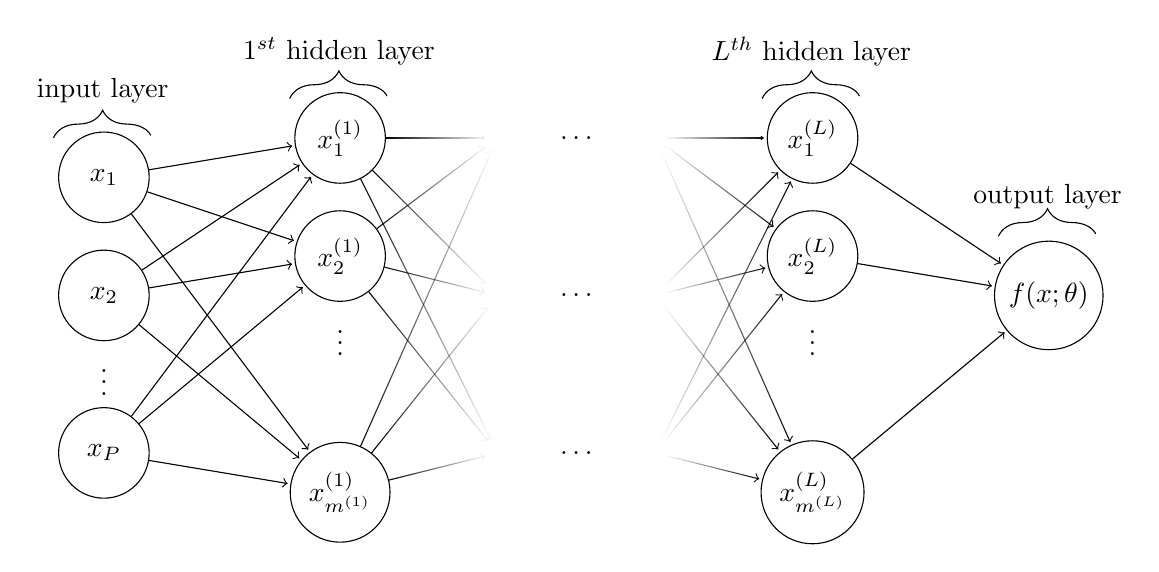
\begin{tikzpicture}[shorten >=1pt]
		\tikzstyle{unit}=[draw,shape=circle,minimum size=1.15cm]
		%\tikzstyle{hidden}=[draw,shape=circle,fill=black!25,minimum size=1.15cm]
		\tikzstyle{hidden}=[draw,shape=circle,minimum size=1.15cm]
 
		\node[unit](x0) at (0,3.5){$x_1$};
		\node[unit](x1) at (0,2){$x_2$};
		\node at (0,1){\vdots};
		\node[unit](xd) at (0,0){$x_P$};
 
		\node[hidden](h10) at (3,4){$x_1^{(1)}$};
		\node[hidden](h11) at (3,2.5){$x_2^{(1)}$};
		\node at (3,1.5){\vdots};
		\node[hidden](h1m) at (3,-0.5){$x_{m^{(1)}}^{(1)}$};
 
		\node(h22) at (5,0){};
		\node(h21) at (5,2){};
		\node(h20) at (5,4){};
		
		\node(d3) at (6,0){$\ldots$};
		\node(d2) at (6,2){$\ldots$};
		\node(d1) at (6,4){$\ldots$};
 
		\node(hL12) at (7,0){};
		\node(hL11) at (7,2){};
		\node(hL10) at (7,4){};
		
		\node[hidden](hL0) at (9,4){$x_1^{(L)}$};
		\node[hidden](hL1) at (9,2.5){$x_2^{(L)}$};
		\node at (9,1.5){\vdots};
		\node[hidden](hLm) at (9,-0.5){$x_{m^{(L)}}^{(L)}$};
 

		\node[unit](y2) at (12,2){$f(x;\theta)$};
 
		\draw[->] (x0) -- (h11);
		\draw[->] (x0) -- (h1m);
		\draw[->] (x0) -- (h10);
 
		\draw[->] (x1) -- (h11);
		\draw[->] (x1) -- (h1m);
		\draw[->] (x1) -- (h10);
 
		\draw[->] (xd) -- (h11);
		\draw[->] (xd) -- (h1m);
 		\draw[->] (xd) -- (h10);
 		
		\draw[->] (hL0) -- (y2);
 
		\draw[->] (hL1) -- (y2);
 
		\draw[->] (hLm) -- (y2);
 
		\draw[->,path fading=east] (h10) -- (h21);
		\draw[->,path fading=east] (h10) -- (h22);
		\draw[->,path fading=east] (h10) -- (h20);
		
		\draw[->,path fading=east] (h11) -- (h21);
		\draw[->,path fading=east] (h11) -- (h22);
		\draw[->,path fading=east] (h11) -- (h20);
		
		\draw[->,path fading=east] (h1m) -- (h21);
		\draw[->,path fading=east] (h1m) -- (h22);
		\draw[->,path fading=east] (h1m) -- (h20);
		
		\draw[->,path fading=west] (hL10) -- (hL0);
		\draw[->,path fading=west] (hL11) -- (hL0);
		\draw[->,path fading=west] (hL12) -- (hL0);
		
		\draw[->,path fading=west] (hL10) -- (hL1);
		\draw[->,path fading=west] (hL11) -- (hL1);
		\draw[->,path fading=west] (hL12) -- (hL1);
		
		\draw[->,path fading=west] (hL10) -- (hLm);
		\draw[->,path fading=west] (hL11) -- (hLm);
		\draw[->,path fading=west] (hL12) -- (hLm);
		
		\draw [decorate,decoration={brace,amplitude=10pt},xshift=-4pt,yshift=0pt] (-0.5,4) -- (0.75,4) node [black,midway,yshift=+0.6cm]{input layer};
		\draw [decorate,decoration={brace,amplitude=10pt},xshift=-4pt,yshift=0pt] (2.5,4.5) -- (3.75,4.5) node [black,midway,yshift=+0.6cm]{$1^{\text{st}}$ hidden layer};
		\draw [decorate,decoration={brace,amplitude=10pt},xshift=-4pt,yshift=0pt] (8.5,4.5) -- (9.75,4.5) node [black,midway,yshift=+0.6cm]{$L^{\text{th}}$ hidden layer};
		\draw [decorate,decoration={brace,amplitude=10pt},xshift=-4pt,yshift=0pt] (11.5,2.75) -- (12.75,2.75) node [black,midway,yshift=0.5cm]{output layer};
	\end{tikzpicture}
	\caption[Multilayer perceptrons with $(L+1)$-layers]{Multilayer perceptrons with $(L+1)$-layers with $P$ input features and 1 output. The $l^{\text{th}}$ hidden layer contains $m^{(l)}$ hidden neurons.}
	\label{fig:multilayer-perceptron}
\end{figure}

So the MLPs is not like classical linear regression in section \ref{LSM} where a single linear transformation from input to output is applied. The unique attribute of neural network is the ability to approximate any kind of function (Universal Apporximate Theorem page 194 \parencite{Goodfellow-et-al-2016}), because of the flexiblility with applying multiple functions to the input layer. The neural network has a lot of different design options, where e.g. hidden layers, layer width, deepth, activation functions etc. are hyperparameters. To fit a model we need to initial weights, initial bias and an activation function for each layer. In order to measure the performance of the model, we need a function to measure the difference the approximation $f(\bm{x};\bm{\theta})$ and the target value $f^*(\bm{x})$. This function is referred as the loss function, where the cost function is the average over the loss functions. The cost function tells us how close predicts $f(\bm{x};\bm{\theta})$ the target y. The cost function is key to improving our model or in machine learning lingo training the model, hence the next section will cover model training \parencite{Goodfellow-et-al-2016}.

%-----------------------------------
%	SUBSECTION 3
%-----------------------------------





\subsection{Training the Network}


Training is essential function minimization where you search in the weightspace that produce a functiont that fit training data well. Objective function to measure how the given weights perform.
Quantifying loss
Gradients is essential for model optimization
stepwidth is our learning rate
we want to minimize the loss with an optimization algorithm to find the optimal set of weights

In general it is recommended to use too many hidden covariates (neurons) rather than too few, and instead introduce some kind of penalty to avoid that the model becomes overly large.
\\
The estimation goal is to minimize a function on the form
$$Q(\theta) = \sum_{i=1}^n L(x_i, \beta^T z^{(L)})$$
where the loss function $L$ often is quadratic.\\
An alternative is to minimize the negative of the log likelihood. \textbf{This is what done in classification.}
A method to estimate the parameters is the gradient descent or the stochastic gradient descent. Here it is necessary to compute the gradient of the objective function. The most common way of doing so is the backpropagation algoritm. This is a forward-backward algorithm. Different starting values of $\theta$ will result in different parameters. The good news is that these predictors typically do not differ by very much. It is recommended to one should work with a set of different starting values, and then use as a final predictor the average of the individual predictors stemming from each starting value. It is also possible to use bagging.
\\
Important to standardize the covariates. And highly correlated covariates should be trimmed down.\\
It is also a good idea to standardize the hidden covariates as well. This is called batch normalization and can accelarate the training of a network considerably.
\\
It is recommended to use batch normalization  in combination with dropout.
\\
It is possible to use ridge or lasso like penalty.
\\
\\
A method that is good at improving the quality is dropout. The idea of dropout is that in the estimation, when updating the gradient, each node is kept with probability $p$, independently of each other. This is a regularization tool.\\

The last update to the output layer is just linear regression\\
The advantage of a multi-layer model is that for each layer the updated set of covariates can be more finely tuned to better explain the data. 

\subsubsection{Backpropagation}
The chain rule: $\frac{dz}{dx}= \frac{dz}{dy} \frac{dy}{dx}$
coputational graph - local gradient -> gradient, because we want to minimize the loss function
so we want $\frac{\partial Loss}{\partial x}$ use chain rule to find the "final gradient".
SO three steps:
1. forward pass: compute Loss
2. compute local gradients
3. backward pass: compute $\dfrac{\partial Loss}{\partial weights}$ using chain rule

%-----------------------------------
%	SUBSECTION 4
%-----------------------------------
\subsection{Regularization}
Overfitting. generalize performance adversed affected.
early stopping

Dropout


The unique attribute of neural network is the ability to approximate any kind of function (Universal Apporximate Theorem), because of the flexiblility with applying multiple functions to the input layer. The neural network has a lot of different design options, where e.g. hidden layers, layer width, activation functions etc. are hyperparameters.


%----------------------------------------------------------------------------------------
%	SECTION 2
%----------------------------------------------------------------------------------------

These network of models are called feedforward because the information only travels forward in the neural network, through the input nodes then through the hidden layers (single or many layers) and finally through the output nodes. 

